\documentclass[11pt]{exam}
\usepackage[activeacute,spanish]{babel} % Permite el idioma espa\~nol.
\usepackage[latin1]{inputenc}
\usepackage{amsmath,amsfonts}
\usepackage[colorlinks]{hyperref}
\usepackage{graphicx}

\pagestyle{headandfoot}

\spanishdecimal{.}

\begin{document}

\firstpageheadrule
%\firstpagefootrule
%\firstpagefooter{}{Pagina \thepage\ de \pages}{}
\runningheadrule
%\runningfootrule
\lhead{\bf\normalsize Taller Python 2018}
\rhead{\bf\normalsize Tarea \'area F\'isica}
\cfoot{ }
\lfoot{\tiny GR}
\begin{flushleft}
\vspace{0.2in}
%\hbox to \textwidth{Nombre: \enspace \hrulefill}
%Nombre : \\
\vspace{0.25cm}
\end{flushleft}
%%%%%%%%%%%%%%%%%%%%%%%%%%%%%%%%%%%%%%%%%%

\begin{center}
\textbf{Fecha M'axima de entrega: Viernes 12 de Enero}
\end{center}
\textbf{Instrucciones:} Resuelva el problema propuesto usando Python. Env'ie todos los archivos necesarios para reproducir sus resultados (archivos de datos, c'odigos .py, notebooks .ipynb, etc.) por email a \texttt{grubilar@udec.cl}.

\bigskip


 Desde el sitio del \textit{Supernova Cosmology Project} (SCp,
\url{http://supernova.lbl.gov/}), descargue el archivo de datos  \url{http://supernova.lbl.gov/Union/figures/SCPUnion2.1_mu_vs_z.txt}.
Este archivo compila la informaci'on del \textbf{redshift} ($z$, segunda columna) y el \textbf{m'odulo de distancia}, que es una medida de distancia usada en Astronom'ia, (tercera columna), junto con su respectivo error (cuarta columna) medidos para cientos
de supernovas\footnote{La primera columna es el nombre o denominaci'on de
la supernova, las otras columnas no son relevantes en este problema.}.
La relaci'on entre el m'odulo de distancia ($\mu$, tambi'en denotado como $m-M$) y el redshift ($z$) de estas
supernovas muy distantes determina el modo en que el Universo evoluciona a escalas cosmol'ogicas. En particular, el hecho que el m'odulo de distancia aumente con el redshift indica que el Universo est'a en expansi'on. 

\begin{parts}
\item Grafique $\mu$ versus $z$ en escala lineal, incluyendo el error en las medidas de $\mu$, y exporte el resultado a un archivo .pdf. El resultado debiese ser similar a al figura \ref{3}, con la diferencia que su gr'afico ser'a a'un m'as hermoso, ya que incluir'a t'itulo, una grilla, as'i como marcadores y colores distintos.
\begin{figure}[ht]
\centerline{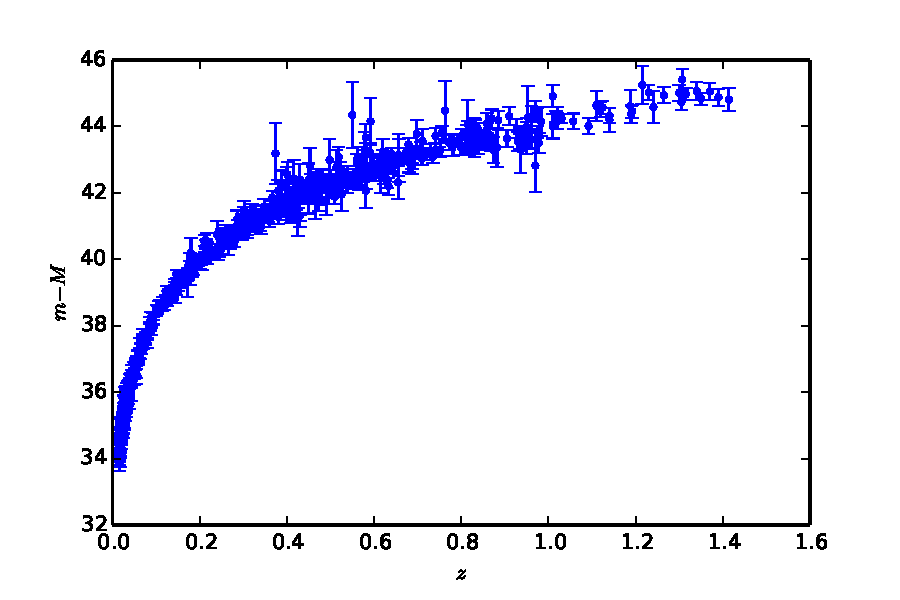
\includegraphics[width=10cm]{figs/m-M-versus-z-con-error.pdf}}
 \caption{M'odulo de distancia versus redsfhift. Escala lineal.}
\label{3}
\end{figure}

\item Modifique su c'odigo anterior para que adem'as exporte el gr'afico de los mismos datos, pero en escala logar'itmica para el redshift $z$ (es decir, el eje horizontal). Este gr'afico debiese ser una versi'on mejorada del de la figura \ref{4}.
\begin{figure}[ht]
\centerline{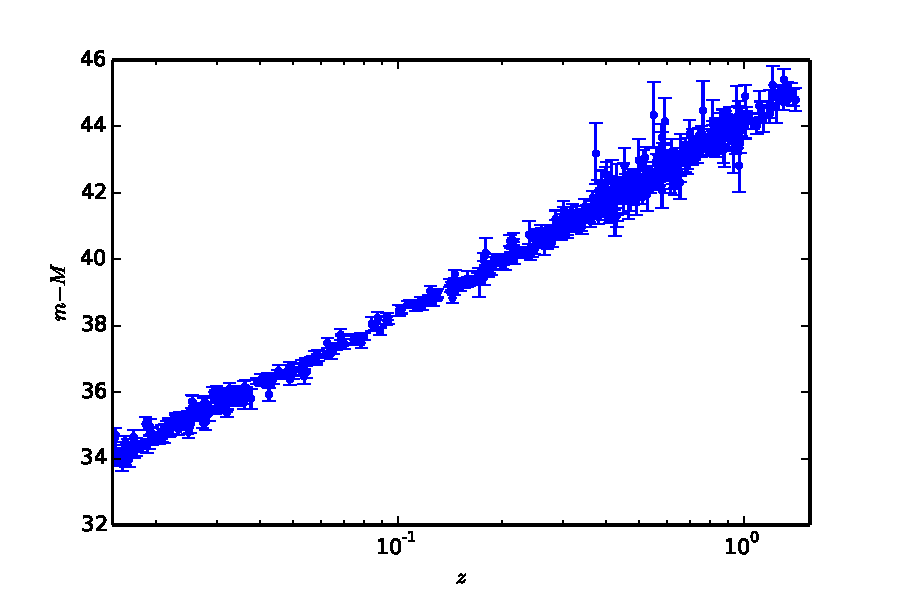
\includegraphics[width=10cm]{figs/m-M_vs_z_semilog.pdf}}
 \caption{M'odulo de distancia versus redsfhift. Escala semilogar'itmica.}
\label{4}
\end{figure}
\item De acuerdo al ``modelo cosmol'ogico est'andar''\footnote{que asume bastantes hip'otesis que simplifican el modelo.}, si la expansi'on se produce a una \textit{tasa constante} entonces la relaci'on entre el redshift $z$ y el m'odulo de distancia $\mu = m-M$ deber'ia ser de la forma
\begin{equation}\label{ec}
\mu=a\cdot \log(z)+b,
\end{equation}
donde $a$ y $b$ son constantes. A partir de esta informaci'on, realize un ajuste del modelo dado por la expresi'on \eqref{ec} y encuentre los valores de $a$ y $b$ que mejor se ajustan a los datos.
\item Confeccione un gr'afico $\mu$ versus $z$ (escala lineal) junto con la funci'on determinada por el ajuste.
\end{parts}


\end{document} 
